\documentclass[onecolumn]{article}
%\usepackage{url}
%\usepackage{algorithmic}
\usepackage[a4paper]{geometry}
\usepackage{datetime}
\usepackage[margin=2em, font=small,labelfont=it]{caption}
\usepackage{graphicx}
\usepackage{mathpazo} % use palatino
\usepackage[scaled]{helvet} % helvetica
\usepackage{microtype}
\usepackage{amsmath}
\usepackage{subfigure}
% Letterspacing macros
\newcommand{\spacecaps}[1]{\textls[200]{\MakeUppercase{#1}}}
\newcommand{\spacesc}[1]{\textls[50]{\textsc{\MakeLowercase{#1}}}}

\title{\spacecaps{FINAL PROJECT:DIABETES }\\ \normalsize \spacesc{CENG 3521, Data Mining} }

\author{Söz Tuana KURŞUN\\Mert Furkan ERGÜDEN\\Mehmet Kubilay ELÜSTÜ\\}
%\date{\today\\\currenttime}
\date{\today}

\begin{document}
\maketitle

\begin{abstract}
In this course and project we learned to write code with the help of some libraries and made it easier.The aim of this course is to classify data and transform it into meaningful data and to reveal valuable data for systems called decision support mechanisms in institutions.With this project, we learned to organize your data set and repair damaged data.Finally,we have observed the most accurate classification with many classification types.In short, we expect the machine to learn.In this way, when new patients arrive, they can be diagnosis by machine learning without examination.
\end{abstract}


\section{Introduction}
In this project we are going to realize, we will predict whether a diabetic patient will be sick or not. Based on the data kept in Excel; it is aimed to segment, group and organize patients.Some information is available in our data set to make this prediction.These are; Pregnancies,	Glucose,Blood Pressure,Skin Thickness,Insulin,BMI,Diabetes Pedigree Function,Age and outcome output. This means that if outcome is 1 so patient is diabetic, 0 if it is not.


\section{Assignments}
If we roughly describe the tasks given in the homework, We will perform various classifications and observe which one gives better results.But with every step we take we have to dig deeper so keep reading :)

\subsection{Assignment1: Editing Data }
First we choose any project, after downloading the project we want, we call it on the command line and we can see the output and go into the details.We see a classification problem because our output consists of 1s and 0s.After calling our set, we call the df.info command to see more detail, so we can see the types and whether they are empty values.Then we check our values with the .isna().sum() command to see if we have missing values.Then we look at our data set to see if there is really missing data? and some things get caught in our eyes, like insulin and glucose values being 0.These values can not be 0 because if they are 0, it means that human is not performing life functions.So what does 0 mean? It means either wrong data or missing data. Since we check the wrong data, these 0's are missing data and to check this, we can look at our data set by calling the .eq(0).sum() command.In order to correct these 0 values, we will write the code in the image and assign NaN values instead of 0s.Thus, we changed our table and then we assigned the average of those values by taking the average of each row instead of NaN values and then rewrite the code we used to check the 0's, so we check our new table and at the end of the part of organizing the data, we wanted to write the code you see in the picture to create a visual feast, so that it appeals to the eye.

\begin{figure}[hb]
\centering
   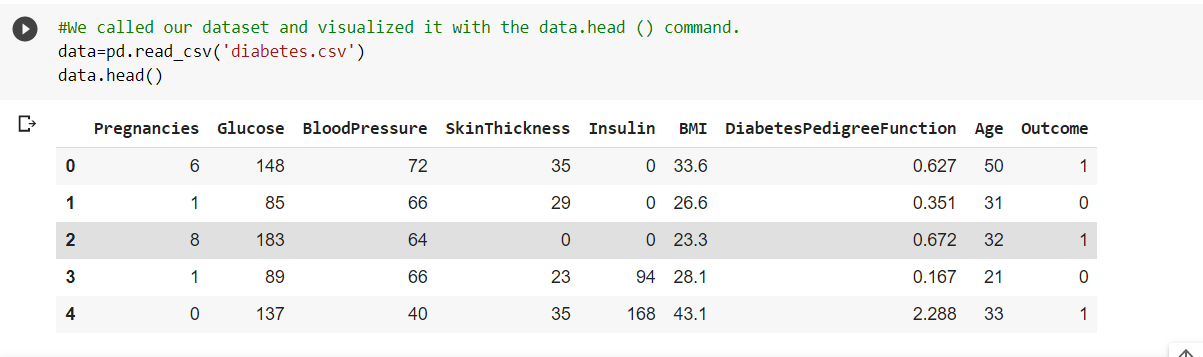
\includegraphics[scale=2,width=.9\linewidth]{head.png}
\caption{\label{fig:code-1}
We called our dataset and visualized it with the data.head () command.}
\end{figure}
\begin{figure}[hb]
\centering
   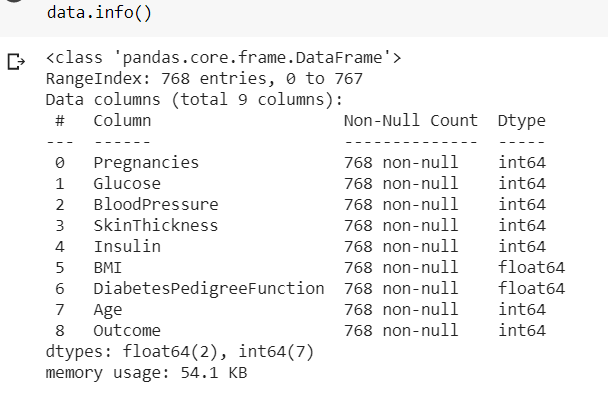
\includegraphics[scale=2,width=.9\linewidth]{info.png}
\caption{\label{fig:code-1}
We decided whether it is true or false by looking at the types in the data set.}
\end{figure}
\begin{center}
    

   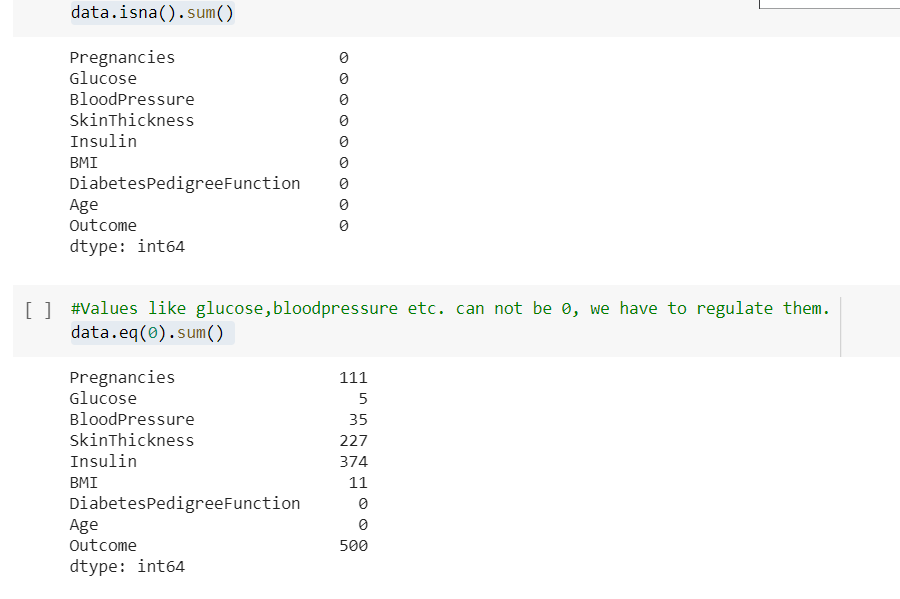
\includegraphics[scale=2,width=.9\linewidth]{double.png}

    \textbf{here we checked if there was an empty data. In the other, we checked the rows whose value is 0.Values like glucose,blood pressure etc. can not be 0, we have to regulate them.}\\
\end{center}

\begin{center}
    

   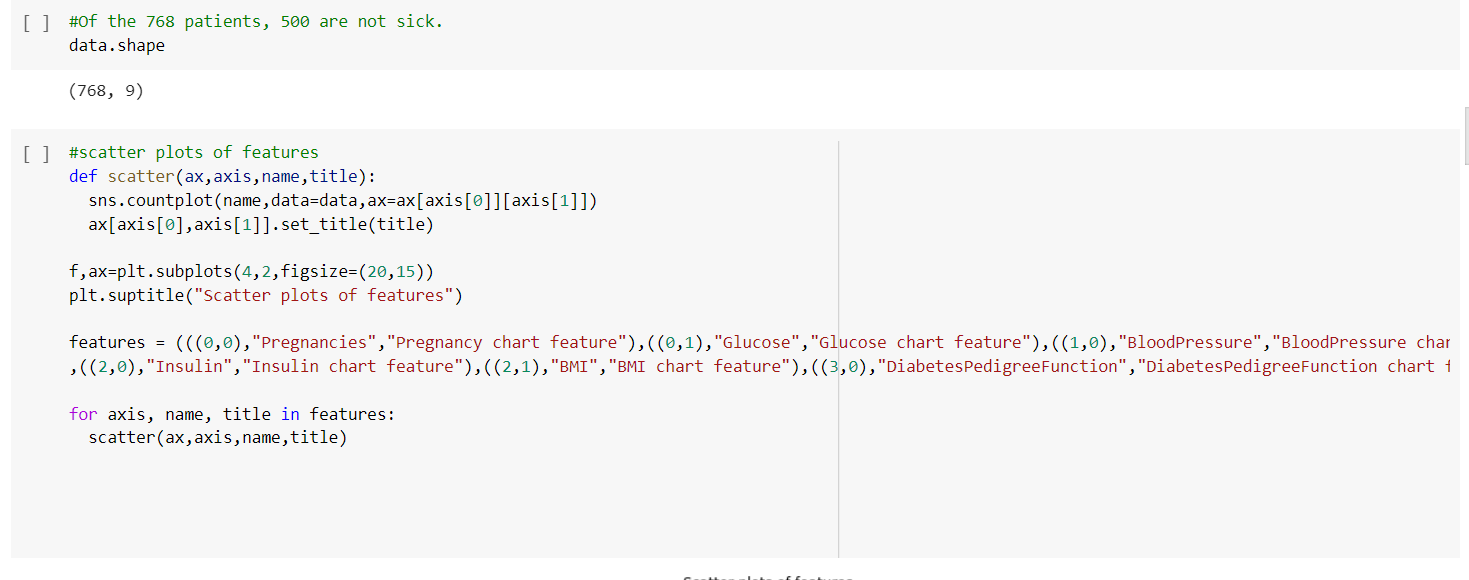
\includegraphics[scale=2,width=.9\linewidth]{scatter.png}

    \textbf{we showed the distribution plots of the features.And the last features for editing data data.shape,this code means we have the 768 patients and 500 are not sick.}\\
\end{center}

\begin{center}
    

   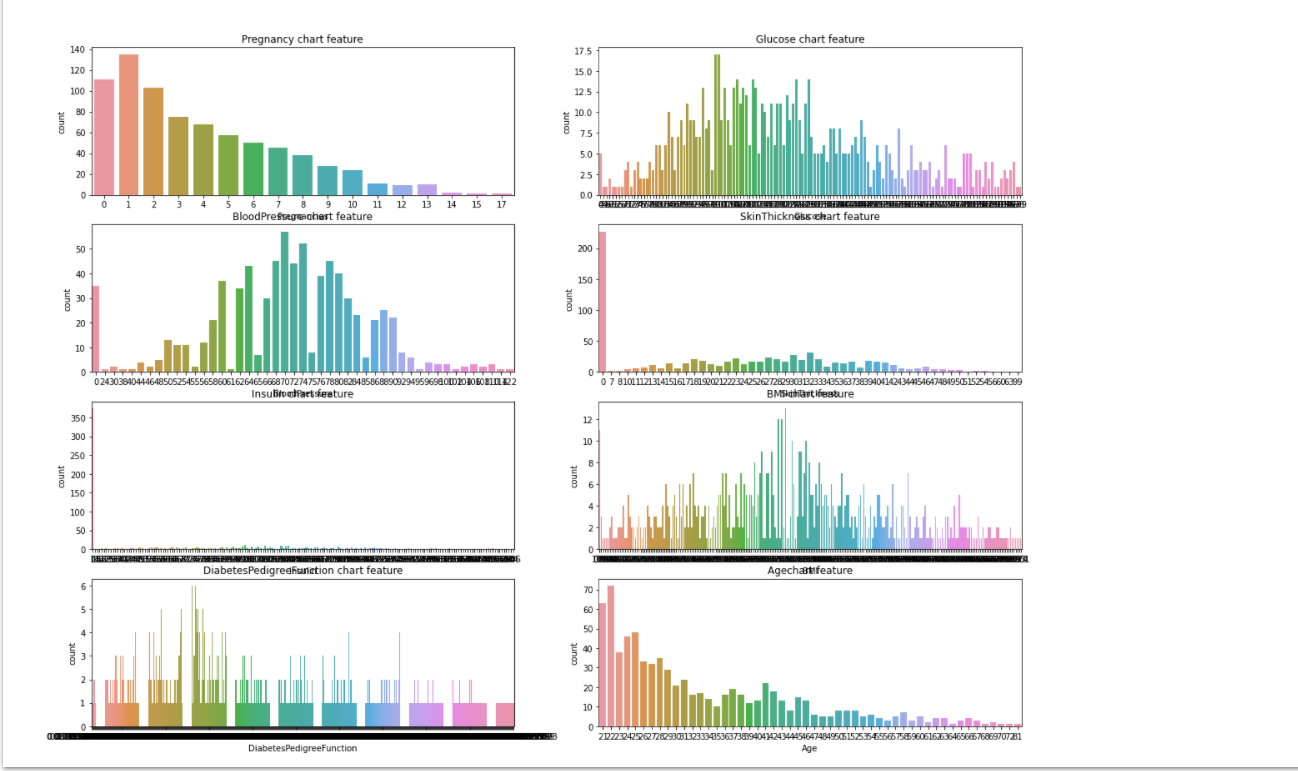
\includegraphics[scale=2,width=.9\linewidth]{image.png}

\end{center}

\begin{center}
    

   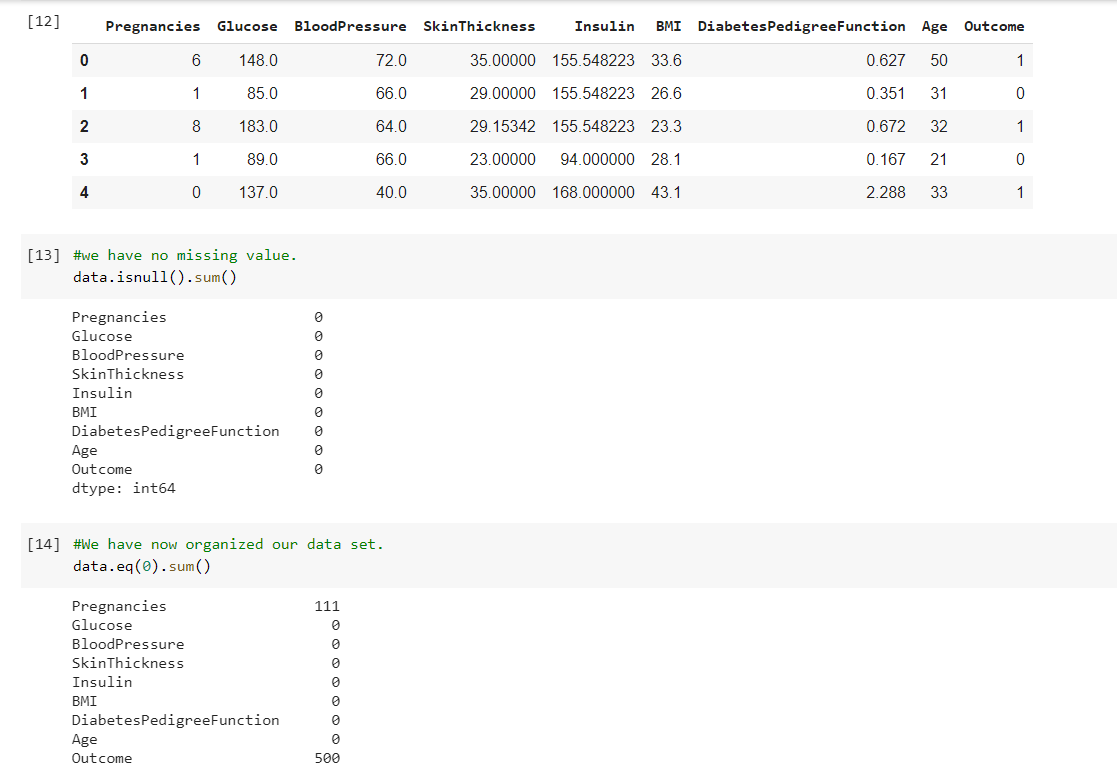
\includegraphics[scale=2,width=1.1\linewidth]{final.png}
    \textbf {We organized all our data and 0 values are filled with means.}

\end{center}

\subsection{Assignment2: Correlation Analysis}
Here we will examine the correlation analysis.What was the correlation? In short, it was the measure of the relationship between two variables.Here we will look at how much the goal affects the output, our outcome value. We can easily call this with a function inside the "pandas." We can see which variables are related to each other through the table. We use the heat map to show it better.
We use the "seaborn" library.

\begin{figure}[hb]
\centering
   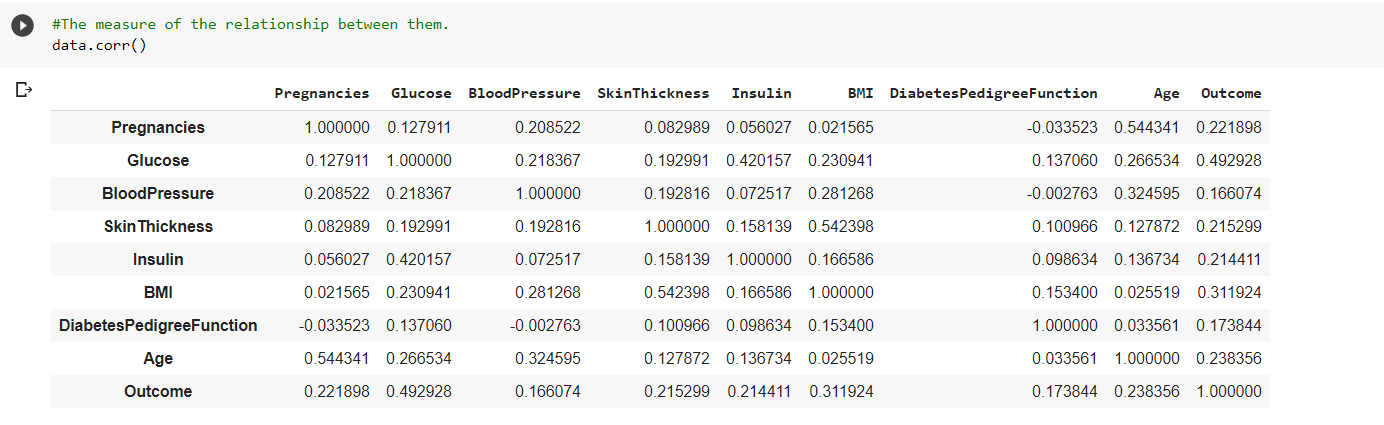
\includegraphics[scale=2,width=.9\linewidth]{corr.png}
\caption{\label{fig:code-2}
In this table we expect high outcome values.}
\end{figure}
\begin{figure}[hb]
\centering
   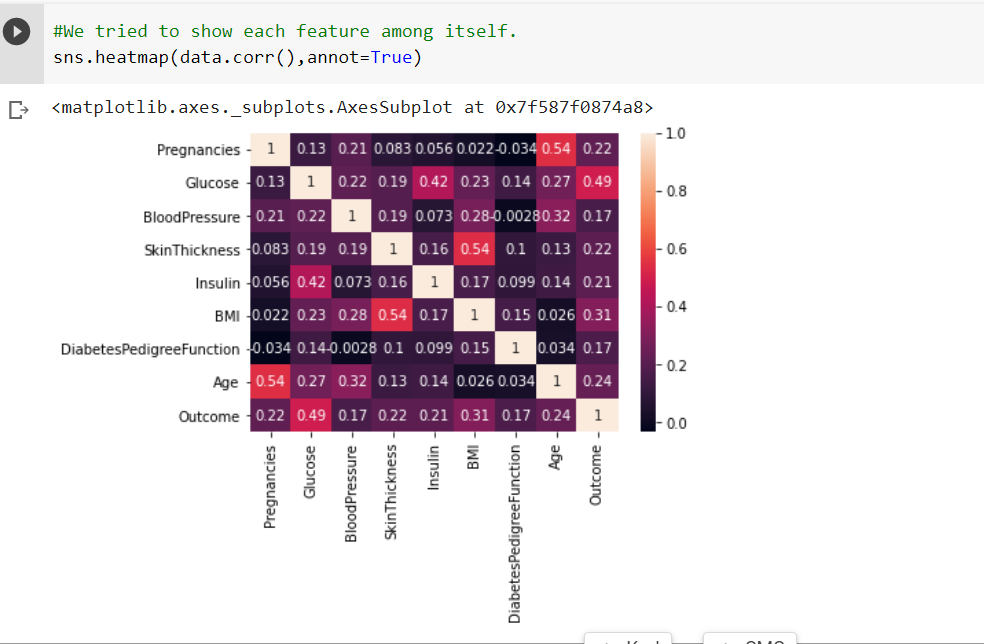
\includegraphics[scale=2,width=.9\linewidth]{heatmap.png}
\caption{\label{fig:code-2}
We tried to show each feature among itself.}
\end{figure}


\subsection{Assignment3: Classification Task }
In the stage, we create the algorithms.We used 3 different types of classification. These are logistic regression,KNN and random forest.Using these three, we chose the classification that gave the closest results and made a performance comparison.We create x and y, and our x values are what we enter and y is our output, that is, outcome.We apply the logistic regression random forest and KNN classifications to our data set, respectively.and we "fit" and "predict" each of them.Finally, we call the score and print the accuracy results on the screen.The more output in the score, the higher our prediction rate.
\\NOTE: Operations will appear in more detail in the code we write.


\subsection{Assignment4: Compare Performance }

In the last task, we compared performance between classifiers and saw which one gave more positive results.We had it plotted with pyplot.plot and we saw the result.

\begin{center}
    

   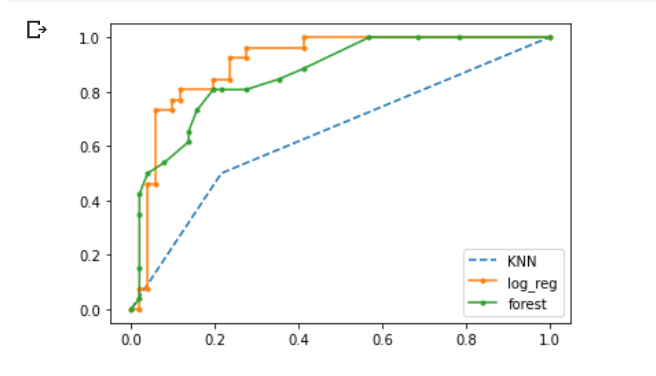
\includegraphics[scale=2,width=.6\linewidth]{compare.png}
  
\textbf{This is the most efficient analysis method, as the most area is under logistic regression.}
\end{center}

\subsection{Assignment5: Sub-tasks Requested From Us }
First, we made clustering in our project, the purpose of which is that we made predictions about outcome, that is, diabetes or not, by connecting with other features without knowing the output,and then we printed the accuracy score.
And then we write the codes for the importance order of the features that trigger diabetes and then drew them.Thus, we see which feature affects diabetes more.(is glucose)The last sub-task was to replace miss data, ie: data with 0 output, with linear regression.By doing Linear regression, we filled the 0 values ​​once with mean, and this time we changed it by regression.

\section{Results}
As a result, we chose the health area, which is a frequently used area in our project. And we edited our data before taking action for forecast results.Since all our data is numerical, it has been easier and more efficient for us.We scanned missing or incorrectly entered data and corrected them, if any.After all our compilation processes were completed, we also had the heatmap drawn and visualized the relationships between them.After these processes were finished, we came to the actual process and created the algorithms and using the information we learned at the beginning of the data mining lesson here we expect the machine to learn.In this way, when new patients arrive, they can be diagnosis by machine learning without examination.

\newpage

\section{Conclusion}

As a result, at the end of this assignment, as I mentioned at all stages,everything gets easier with machine learning. We make our lives easier with machine learning, especially in areas that are important such as health and where processes take time.Instead of doing a lot of tests as in the past, we can find out whether people are diabetes or not by looking at a few features, at least what we say is valid for this project.

\nocite{*}
\bibliographystyle{plain}
\bibliography{references}
\end{document}

